%%%%%%%%%%%%%%%%%%%%%%%%%%%%%%%%%%%%%%%%%%%%%%%%%%%%%%%%%%%
% Organización del proyecto
\section{Organización del proyecto}\label{organizacion:organizacion-del-proyecto}

Dado que el proyecto será manejado por personas en distintos sistemas operativos es vital mantener una coherencia en los nombres y la estructura de los archivos y directorios del proyecto. El presente apartado contiene una propuesta base que considera el funcionamiento general del desarrollo y la estructura de los archivos dentro del repositorio.

\subsection{Organización de carpetas}\label{organizacion:arreglo-carpetas}

\begin{itemize}
\item \textbf{Design:} Esta carpeta contiene todos los archivos del diseño de arte del juego (música, sonidos, sprites, tilesets, bocetos, dibujos, animación, etc.). Es de uso para artistas y desarrolladores y su organización muy probablemente se irá modificando en el tiempo. \emph{Ningún archivo dentro de esta carpeta debe ser referenciado por el código}, por lo mismo permite mayor libertad para ajustar nombres y ubicaciones. Más información al respecto en el apartado \nameref{organizacion:nombres-de-archivos}.

\item \textbf{addons:} Carpeta creada por \lsc{GUT} (unittest) y otros plugins de Godot.

\item \textbf{docs:} Contiene toda la documentación de librerías, licencias, \lsc{API}, \lsc{SDK}, manuales, ToDo, apuntes, notas de compilación y configuración relevante para el desarrollo del software.

\item \textbf{export:} Contiene binarios para distintas plataformas del juego y librerías necesarias para su compilación (Por ejemplo librerías propietarias para generar los binarios de una consola).

\item \textbf{locales:} Contiene todos los ficheros relativos a la i18n. Es la carpeta que utilizarán los traductores y desde donde el juego debe tomar todos los strings y los assets correspondientes (assets con texto).

\item \textbf{src:} Probablemente la carpeta principal para el desarrollo técnico. Además del código fuente del programa contendrá todo lo relativo a nodos, escenas, assets, librerías y scripts. La estructura de esta carpeta será utilizada por el proyecto dentro de Godot.

Una consideración importante para mantener la organización de los archivos de una forma que sea coherente con la abstracción de \textit{escenas y nodos}, es crear cada escena dentro de su propia carpeta. Aquí, además del archivo \lsc{TSCN}, deberían estar todos los assets que utiliza la escena para evitar cualquier problemas de dependencias. La idea es poder mover o copiar la carpeta de ubicación y que todo siga funcionando dentro de ella.

\begin{lstlisting}
$ ls src/characters/player/tyanka/
animations/
    tyanka_walk_01.png
    tyanka_walk_02.png
    tyanka_jump_01.png
    etc.
portraits/
    tyanka_portrait_angry_01.png
    tyanka_portrait_angry_02.png
    tyanka_portrait_happy_01.png
    etc.
powers/
    animal_spirit.gd
    palin_shield.gd
    palin_whirl.gd
    etc.
tyanka.gd
tyanka.tsc
tyanka_stats.json
\end{lstlisting}

Si muchas escenas están utilizando los mismos sprites, probablemente se trate de archivos que deberían procesarse e ir dentro de la carpeta \textbf{shared} (detallada más adelante).

A continuación la organización preliminar de la carpeta \textbf{src}:

\begin{itemize}
	\item \textbf{characters:} Contiene las subcarpetas \lsc{FSM}, enemies, npc y player.

	\item \textbf{game:} Todo lo relativo a los Managers, lógica y mecánicas del juego.

	\item \textbf{items:} Todo lo relativo a ítems. A priori dividir en armors, utility y weapons.

	\item \textbf{levels:} Escenas de niveles organizadas en distintas subcarpetas. Contemplar una ubicación para diversos templates.

	\item \textbf{ui:} Todo lo relativo a las escenas de la interfaz gráfica.
\end{itemize}

\item \textbf{shared:} Colección de todos los assets y resources compartidos por más de una escena. Por ejemplo: fuentes tipográficas, música, tilesets, sprites, assets genéricos, etc.
\end{itemize}

\subsubsection*{Diagrama del árbol de directorios.}
\begin{figure}[H]
\centering
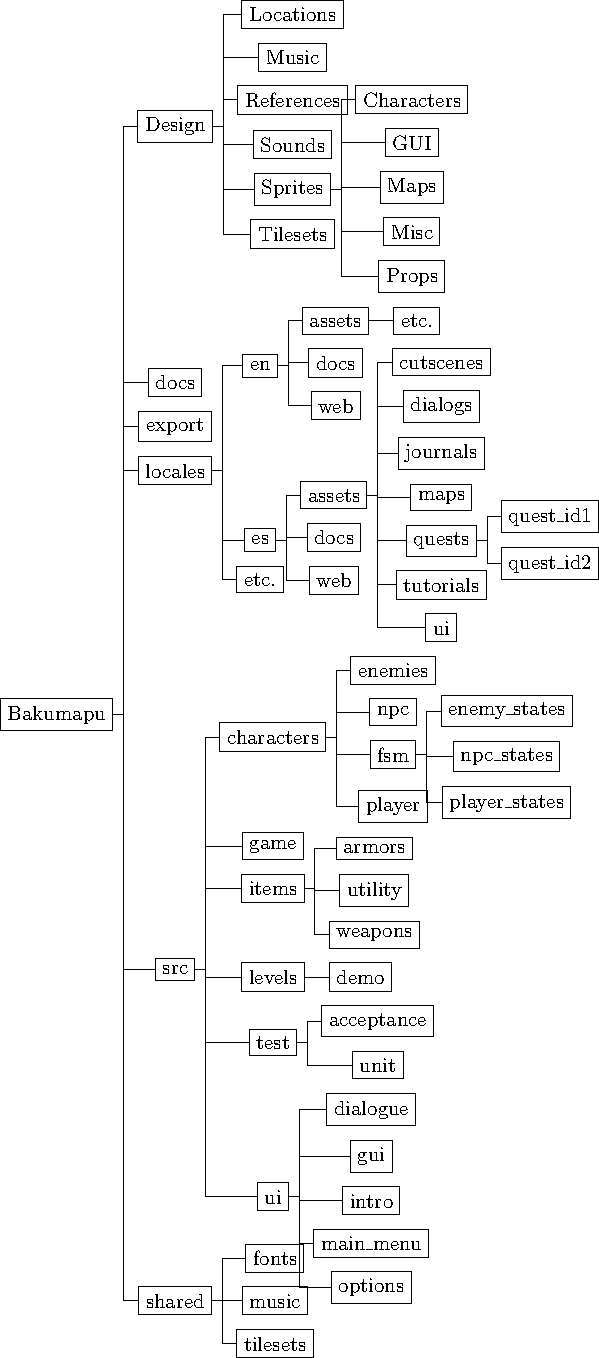
\includegraphics[height=0.93\textheight]{imágenes/arbol_proyecto}
\label{fig:arbolproyecto}
\end{figure}

%%%%%%%%%%%%%%%%%%%%%%%%%%%%%%%%%%%%%%%%%%%%%%%%%%%%%%%%%%%
%%%%%%%%%%%%%%%%%%%%%%%%%%%%%%%%%%%%%%%%%%%%%%%%%%%%%%%%%%%

\subsection{Nombres de archivos}\label{organizacion:nombres-de-archivos}

En términos generales estas son las consideraciones importantes:

\begin{enumerate}
  \item Los nombres solo podrán contener letras \textbf{a-z}, números \textbf{0-9} y guión medio “\textbf{-}” y bajo “\textbf{\_}”. No deberán contener acentos, ni eñe, ni espacios.
  
  \item Todos los nombres de archivos deben estar en inglés.
  
  \item Por compatibilidad, todos los nombres deben estar en minúscula y seguir el estilo \href{https://en.wikipedia.org/wiki/Snake_case}{snake\_case} (palabras en minúscula separadas por guiones bajos “\_”).
\end{enumerate}

La carpeta Design tendrá mayor libertad en los nombres ya que los archivos no serán referenciados por el código; no obstante se sugiere seguir los mismos principios para evitar problemas de pérdida de datos.

%%%%%%%%%%%%%%%%%%%%%%%%%%%%%%%%%%%%%%%%%%%%%%%%%%%%%%%%%%%
%%%%%%%%%%%%%%%%%%%%%%%%%%%%%%%%%%%%%%%%%%%%%%%%%%%%%%%%%%%

\subsection{Nombres de ramas y tarjetas}\label{organizacion:nombres-de-ramas}

\subsubsection{Ramas principales}\label{organizacion:ramas-principales}

La rama \textbf{develop} mantendrá siempre el mismo nombre. Por su parte las ramas \textbf{main} y \textbf{release} seguirán la nomenclatura del versionado semántico, en este caso \textbf{Bakumapu\_vX.Y.Z} donde cada número representa:

\begin{itemize}[label=-]
	\item \textbf{X:} La versión principal. 0 alfa, 1 release. Si hay cambios no compatibles con la versión anterior, \textbf{X} se incrementa en 1.
	
	\item \textbf{Y:} La versión menor. Aumenta cuando se agreguen nuevas funcionalidades. Los archivos del usuario (savegames) deben ser siempre compatibles con la versión menor anterior.
	
	\item \textbf{Z:} La versión de patch. Siempre que se solucionen bugs se incrementa. Cuando avance la versión menor o principal vuelve a cero.
\end{itemize}

\subsubsection{Ramas de implementación y tarjetas}\label{organizacion:id-ramas-tarjetas}
\subsection*{\noindent\normalfont\textit{Asignando una ID}}

Como ya se explicó en el apartado \nameref{flujo:flujo-de-trabajo}, lo primero es anotar la tarea a trabajar en una tarjeta dentro del tablero Kanban. Cada tarea tendrá una \lsc{ID} específica que también se utilizará para nombrar la rama correspondiente en el repositorio. De esta forma será bastante sencillo hacer un seguimiento para depurar el código o cuando se evalúe el flujo de trabajo.

Esta \lsc{ID} tendrá 2 partes separadas por un guión “-”. La primera, señalará el tipo de rama del repositorio asociada a la tarea:

\begin{itemize}
\item \textbf{Rama de features (ft):} Cuando se trate de implementar una nueva funcionalidad estamos hablando de una tarea que corresponde a las ramas de features y su nombre \lsc{ID} deberá comenzará con las siglas \textbf{ft-}.

\item \textbf{Rama de bugs (bug):} Cuando se trate de la corrección de un \lsc{BUG}, las siglas serán \textbf{bug-}.

\item \textbf{Refactorización (rfc):} Cuando la tarea se trate de refactorizar código ya implementado, las siglas a utilizar serán \textbf{rfc-}. La refactorización se debe trabajar directamente sobre develop y la \lsc{ID} debe usarse al momento de hacer el commit hacia develop.

\item \textbf{Documentación (doc):} Los cambios en la documentación del repositorio del código usaran las siglas \textbf{doc-}. La nomenclatura no es necesaria para el repositorio de este documento.

\item \textbf{Otros (misc):} Evidentemente el equipo puede evaluar en cualquier momento crear una nueva categoría sin inconvenientes. El único detalle es incluir esta categoría dentro de este mismo apartado. De momento para tareas puntuales se podría utilizar el identificador \textbf{misc-}.
\end{itemize}

La segunda parte de la \lsc{ID} será un contador {n + 1} por cada sigla: ft-1, ft-2, bug-1, rfc-1, ft-42, etc.

 \begin{center}$\ast$~$\ast$~$\ast$\end{center}

Con estos sencillos elementos se pretende organizar el repositorio de tal forma que el flujo de trabajo vaya en línea con los criterios de gestión de una forma expedita y que permita a cualquier miembro del equipo hacer consultas directas al historial del repositorio para así facilitar el uso de herramientas de gestión y visualización de \lsc{GIT}.

%%%%%%%%%%%%%%%%%%%%%%%%%%%%%%%%%%%%%%%%%%%%%%%%%%%%%%%%%%%
%%%%%%%%%%%%%%%%%%%%%%%%%%%%%%%%%%%%%%%%%%%%%%%%%%%%%%%%%%%

\subsection{Godot}\label{organizacion:godot}

\begin{itemize}
\item \textbf{Escenas:} Los nombres de las escenas dentro de Godot comenzarán con mayúscula. Ojo: los nombres \emph{dentro} de Godot \emph{¡no los archivos!}.

\item \textbf{Nodos:} Los nombres de los nodos parent comenzarán con mayúsculas y los nodos sin hijos con minúscula.
\end{itemize}

\noindent Tanto para los nodos como las escenas se recomienda la notación lowerCamelCase.